\chapter{Graveyard}

% **************************** Define Graphics Path **************************
\ifpdf
    \graphicspath{{Graveyard/Figs/Raster/}{Graveyard/Figs/PDF/}{Graveyard/Figs/}}
\else
    \graphicspath{{Graveyard/Figs/Vector/}{Graveyard/Figs/}}
\fi

% \begin{align}
% CIF: \hspace*{5mm}F_0^j(a) = \frac{1}{2\pi \iota} \oint_{\gamma} \frac{F_0^j(z)}{z - a} dz
% \end{align}

% \nomenclature[z-cif]{$CIF$}{Cauchy's Integral Formula}                                % first letter Z is for Acronyms
% \nomenclature[a-F]{$F$}{complex function}                                                   % first letter A is for Roman symbols
% \nomenclature[g-p]{$\pi$}{ $\simeq 3.14\ldots$}                                             % first letter G is for Greek Symbols
% \nomenclature[x-i]{$\oint_\gamma$}{integration around a curve $\gamma$} % first letter X is for Other Symbols
% \nomenclature[r-j]{$j$}{superscript index}                                                       % first letter R is for superscripts
% \nomenclature[s-0]{$0$}{subscript index}                                                        % first letter S is for subscripts

% \begin{enumerate}
% \end{enumerate}
% ...
% \begin{enumerate}\setcounter{enumi}{2}
% \end{enumerate}

% \begin{table}
% \caption{Even better looking table using booktabs}
% \centering
% \label{table:good_table}
% \begin{tabular}{l c c c c}
% \toprule
% \multirow{2}{*}{Dental measurement} & \multicolumn{2}{c}{Species I} & \multicolumn{2}{c}{Species II} \\
% \cmidrule{2-5}
%   & mean & SD  & mean & SD  \\
% \midrule
% I1MD & 6.23 & 0.91 & 5.2  & 0.7  \\

% I1LL & 7.48 & 0.56 & 8.7  & 0.71 \\

% I2MD & 3.99 & 0.63 & 4.22 & 0.54 \\

% I2LL & 6.81 & 0.02 & 6.66 & 0.01 \\

% CMD & 13.47 & 0.09 & 10.55 & 0.05 \\

% CBL & 11.88 & 0.05 & 13.11 & 0.04\\
% \bottomrule
% \end{tabular}
% \end{table}

Every aspiring music theorist is at some point tasked with composing simple
pieces of music in order demonstrate understanding of the harmonic rules of
Western classical music. These pedagogical exercises often include
harmonization of chorale melodies, a task which is viewed as sufficiently
constrained to allow a composer's basic technique to be judged. A generative
model for music scores can be applied to this task by conditioning on the
melody line and sampling the conditional distribution for possible
harmonizations.

A more difficult task is automatic composition, where the composer is tasked
with producing an original composition of a particular musical style. The open
nature of this task enables a composer to demonstrate both their
understanding of music theory as well as their creativity. However, this lack of
constraints and loose definition of musical style makes it more difficult to
evaluate the quality of the output. To apply a generative model towards this
task, we can train the model to assign larger probability mass to stylistically
similar scores and then sample the model to generate a novel composition.



\section{Neural Networks}

A common choice is the logistic function $\sigma(z)
= \frac{1}{1+\exp{-z}}$, which squashes $\vec{y} \in [0, 1]$. Other choices
include $\sigma = \tanh$, in which case $[L, U] = [-1, 1]$.

It is common to represent feedforward neural networks as directed acyclic
graphs (\mynote{CITE: fig:nn-layer}). Here, each node denotes a data value and
an edge from $s$ to $t$ notates that the value at $s$ is used to compute the
value at $t$.

\begin{figure}[tb]
    \centering
    \def\layersep{2.5cm}

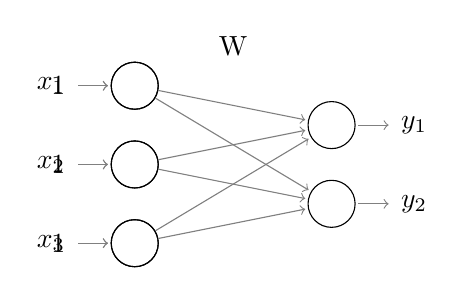
\begin{tikzpicture}[shorten >=1pt,->,draw=black!50, node distance=\layersep]
    \tikzstyle{every pin edge}=[<-,shorten <=1pt]
    \tikzstyle{neuron}=[circle,draw=black!100, minimum size=17pt,inner sep=0pt]
    \tikzstyle{input neuron}=[neuron];
    \tikzstyle{output neuron}=[neuron];
    \tikzstyle{hidden neuron}=[neuron];
    \tikzstyle{annot} = [text width=4em, text centered]

    % Draw the input layer nodes
    \foreach \name / \y in {1,...,3}
        \ifthenelse{3 = \y}{
            \node[input neuron, pin=left:$1$] (I-\name) at (0,-\y) {};
        }{
            \node[input neuron, pin=left:$x_\y$] (I-\name) at (0,-\y) {};
        }; % (*)

    % Draw the output layer node
    \foreach \name / \y in {1,...,2}
        \path[yshift=-0.5cm]
            node[output neuron,pin={[pin edge={->}]right:$y_\y$}] (O-\name) at (\layersep,-\y cm) {};

    % Connect every node in the input layer with every node in the
    % output layer
    \foreach \source in {1,...,3}
        \foreach \dest in {1,...,2}
            \path (I-\source) edge (O-\dest);

    \node[annot,above of=I-1, xshift=0.5*\layersep, node distance=0.5cm] {W};
\end{tikzpicture}

    \caption{Single feedfoward neural network layer}
    \label{fig:nn-layer}
\end{figure}

Multiple layers can be composed together by treating the outputs from the previous layer
as the inputs to the next layer. \mynote{CITE: fig:ffw-nn} illustrates this on a 2-layer
feedforward neural network where the outputs of the first layer are used as the
inputs to the second layer (\ie $x^{(1)} = y^{(0)}$).


\begin{figure}[htbp]
    \centering
    \def\layersep{2.5cm}

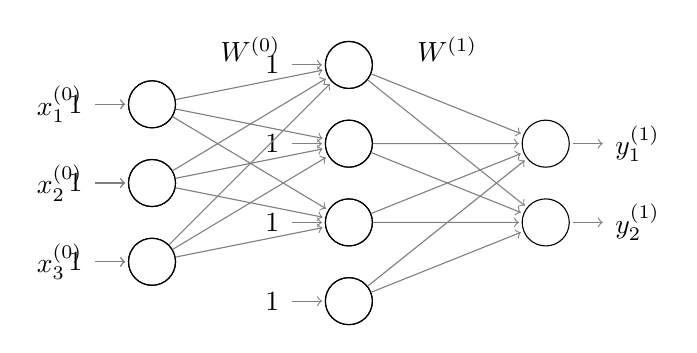
\begin{tikzpicture}[shorten >=1pt,->,draw=black!50, node distance=\layersep]
    \tikzstyle{every pin edge}=[<-,shorten <=1pt]
    \tikzstyle{neuron}=[circle,draw=black!100, minimum size=17pt,inner sep=0pt]
    \tikzstyle{input neuron}=[neuron];
    \tikzstyle{output neuron}=[neuron];
    \tikzstyle{hidden neuron}=[neuron];
    \tikzstyle{annot} = [text width=4em, text centered]

    % Draw the input layer nodes
    \foreach \name / \y in {1,...,3}
        \ifthenelse{3 = \y}{
            \node[input neuron, pin=left:$1$] (I-\name) at (0,-\y) {};
        }{
            \node[input neuron, pin=left:$x^{(0)}_\y$] (I-\name) at (0,-\y) {};
        };

    % Draw the hidden layer nodes
    \foreach \name / \y in {1,...,4}
        \ifthenelse{4 = \y}{
            \path[yshift=0.5cm]
                node[hidden neuron, pin=left:$1$] (H-\name) at (\layersep,-\y cm) {};
        }{
            \path[yshift=0.5cm]
                node[hidden neuron] (H-\name) at (\layersep,-\y cm) {};
        };

    % Draw the output layer node
    \foreach \name / \y in {1,...,2}
        \path[yshift=-0.5cm]
            node[output neuron,pin={[pin edge={->}]right:$y^{(1)}_\y$}] (O-\name) at (2*\layersep,-\y cm) {};

    % Connect every node in the input layer with every node in the
    % hidden layer.
    \foreach \source in {1,...,3}
        \foreach \dest in {1,...,3}
            \path (I-\source) edge (H-\dest);

    % Connect every node in the hidden layer with the output layer
    \foreach \source in {1,...,4}
        \foreach \dest in {1,...,2}
            \path (H-\source) edge (O-\dest);

    % Annotate the layers
    \node[annot,above of=I-1, xshift=0.5*\layersep, node distance=0.7cm] (hl) {$W^{(0)}$};
    \node[annot,right of=hl] {$W^{(1)}$};
\end{tikzpicture}

    \caption{2-layer feedforward neural network}
    \label{fig:ffw-nn}
\end{figure}

When discussing neural networks with $L \geq 1$ layers, we will use
$\vec{x}^{(i)}$, $\matr{W}^{(i)}$, $\vec{z}^{(i)}$, and $\vec{y}^{(i)}$ to
refer to the inputs, weights, activations, and outputs of the $i$th layer. The
activation function $\sigma$ is understood to act elementwise when applied to a
vector. For adjacent layers $i$, $i+1$, we have $\vec{x}^{(i+1)} =
\vec{y}^{(i)}$. $\vec{x}^{(0)}$ and $\vec{y}^{(L)}$ are the inputs and outputs
respectively of the entire network.

The non-linearity introduced by the activation function $\sigma$ is paramount
for enabling neural networks to model a broad variety of functions. \mynote{
    If activation functions are removed, then a neural
network can only model affine transformations.}

\subsubsection{Modeling probability distributions}

A neural network can be used to model the distribution of a categorical random
variable $o$ by treating the final layer activations $\vec{z}^{(L)}$ as the
energies of a Boltzmann distribution (\ie\ $\softmax$). This implies a
probability mass function on $o$ given by \mynote{CITE: eq:softmax}.

\begin{equation}
    \label{eq:softmax}
    P(o = k | \vec{z}^{(L)}) = \frac{\exp{-z^{(L)}_k}}{ \sum_{j} \exp{-z^{(L)}_j} }
\end{equation}

\subsubsection{Efficient graident computations through back-propogation}

Feed-forward neural networks are trained using back-propogation, an efficient
algorithm which consists of a forward pass to compute activations followed by
back-propogation of partial derivatives expanded according to the chain
rule\mynote{cite backprop}. At the heart of back-propogation is the
\textbf{computation graph} of a a model: a directed acyclic graph where each
node represents a differentiable function that can compute its outputs and
Jacobian given inputs and activations\mynote{cite theano}. By representing only
the dependencies between intermediate values, the sparsity imposed by the
computation graph enable back-propogation to ignore irrelevant
cross-derivatives and efficiently compute global gradients from local
computations.


Training of recursive neural networks is typically performed using
backpropogation through time (BPTT)\mynote{Cite}, a technique computationally
equivalent to feedforward training of the unrolled computation graph. This is
easily seen: unrolling of a RNN yields a feed-forward structure where the
standard back-propogation algorithm applies.




\subsubsection{Vanishing gradients}

The solution is to rewrite \mynote{CITE: eq:ht-from-ht-1} such that
\mynote{CITE: eq:prod-hi} does not vanish/explode for large $t - k$.
One possibility would be

\begin{equation}
    h_t = h_{t-1} + \theta_x x_t
\end{equation}

However, this solution is unsatisfactory as all hidden state dynamics have been
removed.


\subsubsection{Training with back-propogation}

Training neural networks is achieved using gradient descent methods, which
optimize parameters $\theta = \{W^{(i)} : 1 \leq i \leq L \}$ to minimize some
loss function $L(\vec{z}^{(L)}_{1:N}, \hat{o}_{1:N})$ between the network
outputs $\vec{z}^{(L)}_{1:N}$ and the true labels $\hat{o}_{1:N}$. For
probabilistic classification, a common choice is to assume independence
across training examples and use \textbf{cross-entropy loss}
(\mynote{CITE: eq:cross-entropy-loss}):

\begin{align}
    L(\vec{z}^{(L)}_{1:N}, \hat{o}_{1:N})
    &= \sum_{i=1}^{N} L(\vec{z}^{(L)}_i, \hat{o}_i) &\text{Independence across samples} \nonumber\\
    &= \sum_i \sum_k \delta_{\hat{o}_i,k} \log \frac{1}{P(o=k | \vec{y}_i^{(L)})} & \label{eq:cross-entropy-loss}
\end{align}

Gradient descent proceeds by using the Jacobian (\ie\ gradient) $\nabla_\theta
L(\vec{z}^{(L)}_{1:N}, \hat{o}_{1:N})$ to iteratively update the network
parameters using successive first-order approximations (\mynote{CITE: eq:nn-training-iteration-scheme}).

\begin{align}
    \label{eq:nn-training-iteration-scheme}
    \theta^{(t+1)} = \theta^{(t)}
    - \eta_t \left[ \nabla_\theta L(\vec{z}^{(L)}_{1:N}, \hat{o}_{1:N}) \right]_{\theta = \theta^{(t)}}
\end{align}

Variants of \mynote{CITE: eq:nn-training-iteration-scheme} which adaptively set the
step size $\eta_t$ or incorporate/estimate the Hessian $\nabla^2_{\theta}
L(\cdot, \cdot)$ can yield performance when applied to neural network training.
However, their discussion is out of scope. \mynote{Discuss RMSprop?}

To apply \mynote{CITE: eq:nn-training-iteration-scheme}, the gradient $\nabla_\theta
L(\vec{z}^{(L)}_{1:N}, \hat{o}_{1:N})$ must be computed. This can be
accomplished using \textbf{backpropogation} \mynote{cite}, an algorithm which
exploits the independence structure to avoid unnecessary computations and make
gradient computations tractable.

Let $\delta^{(l)}_{j} = \frac{\pd L(\vec{z}^{(L)}_{1:N}, \hat{o}_{1:N})}{\pd
z^{(l)}_j}$ be the partial derivative of the loss with respect to the $j$th
activation of layer $l$. For the final $L$th layer, cross-entropy loss
with a Boltzmann distribution yields

\mynote{CITE: eq:cross-entropy-loss}
\begin{align*}
    \delta^{(L)}_{j}
    &= - \sum_{i=1}^{N} \sum_{k} \frac{\pd}{\pd z^{(L)}_j} \delta_{\hat{o}_i,k} \log P(o=k | \vec{z}^{(L)}_i ) &\text{CITE HERE} \\
    &= \sum_{i=1}^{N} \left( P(o=k | \vec{z}^{(L)}_i ) - y_i \right) & \text{Softmax derivative}
\end{align*}

For earlier layers $l < L$, we have
\begin{align}
    \delta^{(l)}_{j}
    &= \sum_k \frac{\pd L(\vec{z}^{(L)}_{1:N}, \hat{o}_{1:N})}{\pd z^{(l+1)}_k}
    \frac{\pd z^{(l+1)}_k}{\pd z^{(l)}_j}\\
    &= \sum_k \delta^{(l+1)}_k
    \frac{\pd}{\pd z^{(l)}_j} \left( \matr{W}^{(l+1)} [\sigma(z^{(l)}), 1]^\tp \right)_k \\
    &= \sum_k \delta^{(l+1)}_k
    \matr{W}^{(l+1)}_{k,j} \sigma'(z^{(l)}_j) \label{eq:backprop}
\end{align}
This expression can be vectorized using the Hadamard product (elementwise multiplication), which
improves performance due to CPU cache locality and coalesced memory loads: \mynote{DO THIS}
\begin{align}
    \circ
\end{align}
This recursion can be iterated until $l \to 0$.

The back-propogation algorithm consists of two steps:
\begin{enumerate}
    \item \emph{Forward pass}: Using current model parameters $\theta^{(t)}$,
        feed the data into the network to compute the activations $\vec{z}^{(l)}$,
        $1 \leq l \leq L$
    \item \emph{Backward pass}: Recursively iterate \mynote{CITE: eq:backprop}
        to compute $\vec{\delta}^{(l)}$, $1 \leq l \leq L$ using the activations
        $\vec{z}^{(l)}$ obtained from the forward pass
\end{enumerate}

After the backwards pass, gradients with respect to model parameters are easily obtained
\begin{align}
    \frac{\pd L}{\pd W^{(l)}_{i,j} }
    &= \sum_k \frac{\pd L}{\pd z^{(l+1)}_k} \frac{\pd z^{(l+1)}_k}{\pd W^{(l)}_{i,j}} \\
    &= \sum_k \delta^{(l+1)}_k z^{(l)}_j
\end{align}

Some appealing properties of backpropogation:
\begin{itemize}
    \item Efficient exploitation of the computation graph: chain rule expansions
        are constrained by the computation graph, improving efficiency
        because factors which don't contribute to a given $\delta^{(l)}$
        are neglected in the recursion
    \item Implementation using local rules: the forward/backward pass
        at any layer $l$ only requires knowledge of $z^{(l)}$, $\delta^{(l+1)}$,
        and the derivative of the activation $\sigma'$. As all these quantities are localized
        to one layer, this permits modular implementations where a node which can be back-propped
        through needs only implement a \texttt{forward()} method which computes activations
        given inputs and a \texttt{backward()} method which computes $\delta^{(l)}$ given
        activations.
\end{itemize}

\mynote{Talk about how localization gives rise to computation graph and autodiff}

\section{RNNs}

The advantages of RNNs over feedforward networks include:
\begin{itemize}
    \item Ability to handle variable-length inputs: the RNN can be unrolled an arbitrary
        number of times to accomodate inputs $\vec{x}$ of different length
    \item Fixed dimension embeddings: after processing the entirety of an input
        sequence, the state of the RNN can be used as a fixed dimension embedding
        representing the input
    \item Sequential processing: the order of $\vec{x}_{1:T}$ will affect the state
        trajectory $s_{1:T}$, enabling the model to capture time-dependent dynamics
        within the input sequences
    \item Memory over time: the state $s \in \RR^D$ can take on an uncountably infinite
        number of values, allowing it to potentially act as memory which summarizes
        \emph{all} of the input up to the current time
\end{itemize}

\subsubsection{Comparison against HMMs}

Hidden Markov Models (HMMs) are another popular probabilistic model for
sequental data. \mynote{Define HMMs}

While RNNs are similar HMMs in that both model the conditional distribution of
next frames given the previous context. However, RNNs additionally pass along
"hidden state" which summarizes contextual information from a potentially
infinite context window.


\begin{figure}[tb]
    \centering
    \input{Graveyard/Figs/lstm-unit.pdf_tex}
    \caption{Single LSTM unit}
    \label{fig:lstm-unit}
\end{figure}


\section{Sequence probability modelling}

Generating a "Bach-like" piece of music can be understood as drawing a random
sample from a distribution over musical scores which is statistically similar
to Bach's own compositions. Thus, we interpret the problem as one of
\emph{categorical sequence modeling}.

This type of problem has been well studied. In speech recognition, language
models parameterizing distributions over sentences are used as priors to refine
transcriptions.

However, since our model has to be able to generate Bach, we must be able to
sample from it. This rules out a broad class of sequence models, including
back-off N-grams and other interpolated language models.

Fortunately, low order N-grams and standard HMM-based models are sampleable and
thus can be used as baselines.

\section{Related work}

\cite{Cuthbert2011} used
\texttt{music21} to generate rich feature representations for music for
downstream machine learning tasks.

The application of machine learning to music has a rich history.
\cite{Herlands2014} describe a system to classify music into homogeneous
styles. However, they focus on the discriminative task and do not consider
how to generate novel scores.

In \emph{Bach in a Box} \cite{spangler1998bach},
harmonic rules are collected in a database and then used to build rule-based
neural networks. This enables encoding of prior knowledge as rules in the
rulebase.



\section{LSTM: background and motivation}

Two prominent methods for training RNNs include real-time recurrent learning (RTRL)
\cite{robinson1987utility} and backpropogation through time (BPTT) \cite{williams1995gradient}.
\cite{williams1990efficient} introduces truncated BPTT to address computational complexity
when learning over very long sequences. Temporal difference \cite{sutton1998reinforcement} has
also been proposed as a method for learning RNNs \cite{franklin2004predicting}.

The first LSTM models, which did not include forget gates, was introduced in
\cite{hochreiter1997long}. \cite{gers2000learning} later revised the LSTM model
to include forget gates in order to prevent hidden states from growing
indefinitely.

LSTM have been demonstrated to outperform traditional RNNs on a variety of
tasks. \cite{gers2001lstm} demonstrates a LSTM correctly recognizing $1000$
instances from the context-free grammar $A^n B^n$ while an Elman RNN achieves
only $20\%$ accuracy.

Online adaptation at test time using a Kalman filter was described in \cite{gers2002dekf}.
\cite{Mikolov2010} \cite{Mikolov2012} refers to this as ``dynamic evaluation.''

\cite{eck2008learning} attempts to model meter by introducing time-delayed
connections in \cite{Eck2002}

\subsection{Representation of music data}

\cite{mozer1994neural} discusses the importance of music representation,
settling on \emph{psychologically-based representations} of pitch, duration,
and harmonic structure \cite{shepard1982geometrical}.

Many attempts to represent musical data have been investigated. Attempts which
explicitly model harmonic structure include a Circle of Thirds representation
\cite{franklin2004recurrent} or overlapping subharmonics
representation\cite{laden1989representation}, both of which have been studied
in the context of generative RNN models \cite{franklin2004recurrent}
\cite{mozer1994neural}. Other representations attempt to model notions such as
musical distance in terms of voice leading, orbifolds, and tuning
lattices\cite{Tymoczko2009}.

\cite{franklin2005jazz} introduce a LSTM model for jazz melodies which use
separate units for notes and their durations.

The success of these methods are varied and it remains ambiguous if any
is better. Furthermore,

\section{Evaluation of models}

\cite{pearce2001towards} addresses difficulty in quantitative evaluation,
suggesting the use of a learned critic in a manner similar to GANs
\cite{goodfellow2014generative}. In a later report,
\cite{pearce2002motivations} attribute difficulty in evaluation due to lack
aim: algorithmic composition, design of compositional tools, and computational
modelling of musical styles or music cognition all have different motivations
and should thus be evaluated differently.

\cite{ariza2009interrogator} criticizes a musical Turing test as providing little data about
how to improve the system, suggesting that listener studies using music experts
may be more insightful.


\section{Token-level embeddings}

\mynote{EXPERIMENT: redo these}

Filter to notes

\begin{figure}[tb]
    \centering
    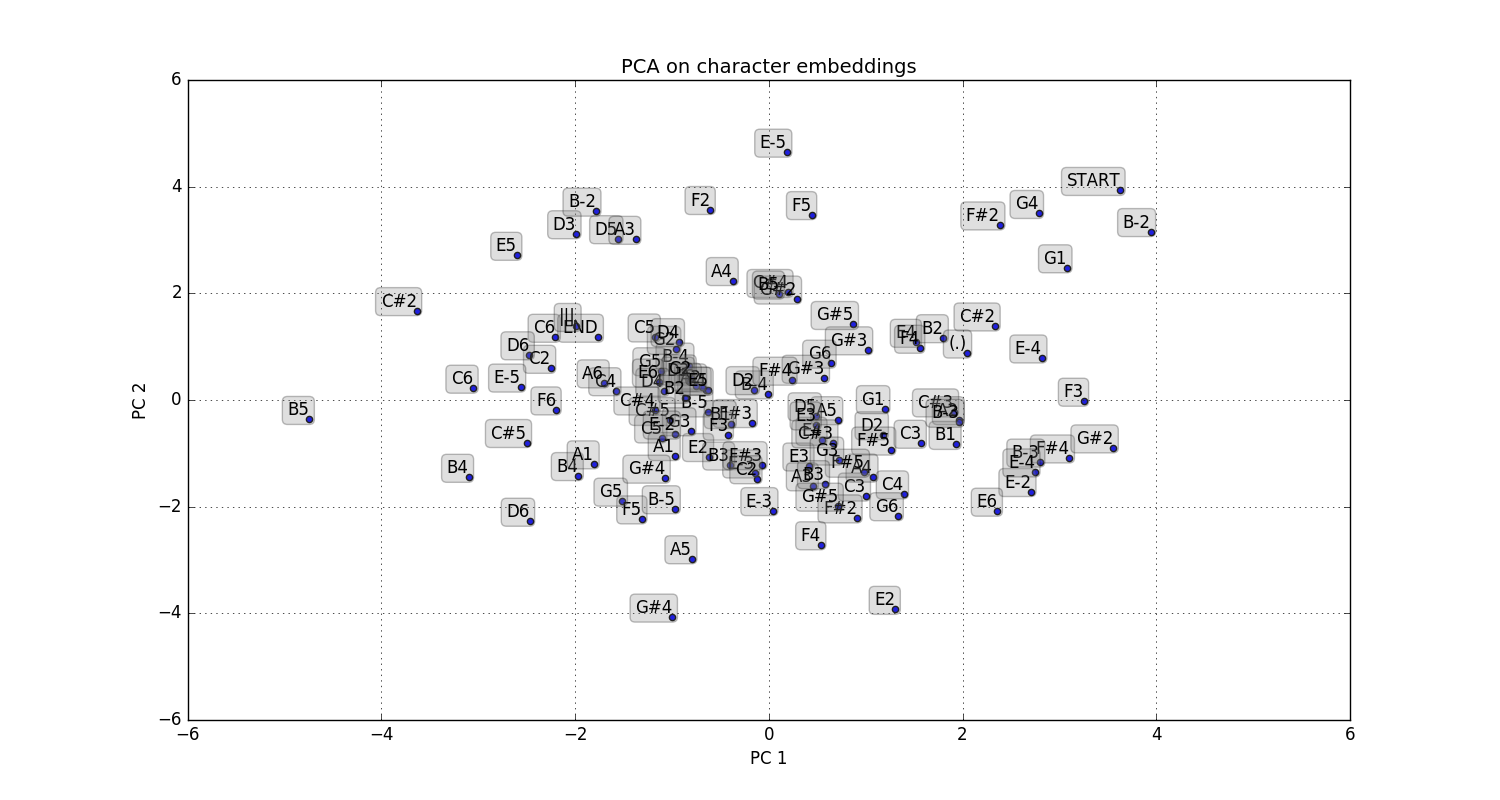
\includegraphics[width=1.0\linewidth]{PCA-notes.png}
    \caption{PCA embedding of note tokens}
    \label{fig:pca-notes}
\end{figure}

\begin{figure}[tb]
    \centering
    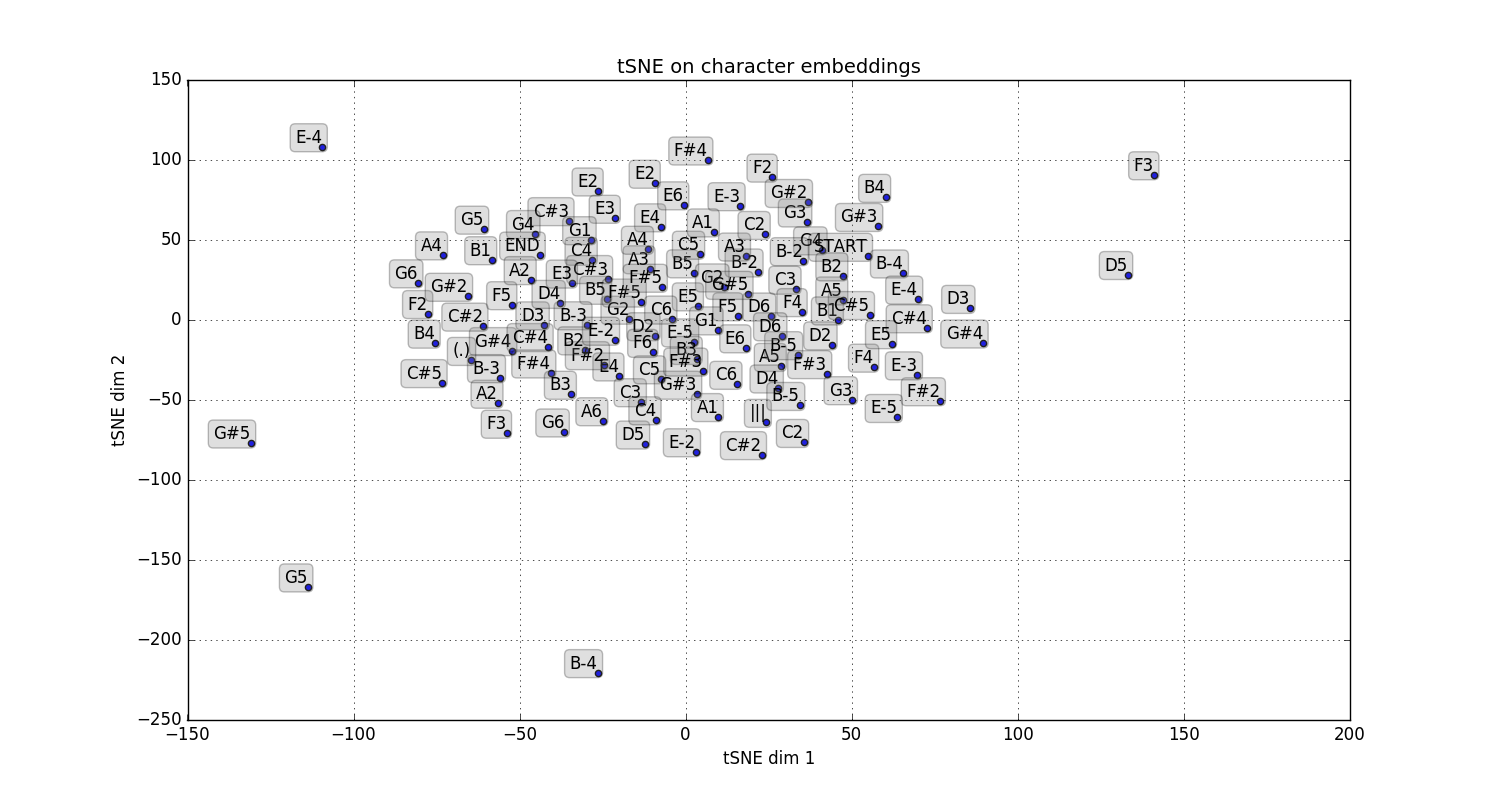
\includegraphics[width=1.0\linewidth]{tSNE-notes.png}
    \caption{tSNE embedding of note tokens}
    \label{fig:tsne-notes}
\end{figure}

\subsection{Variable-length embeddings}

\mynote{EXPERIMENT: LSTM hidden state after consuming chord (chord boundary, do they
    cluster?), phrase (up to fermata, do similar phrases embed similarly),
    whole pieces (difficult to evaluate)}
